% Risultati ottenuti

\chapter{Performance Analysis}
    This chapter characterizes two systems with different types of photon added state in term of
    their discrimination MDEP \ref{eq:HelstromBound}: a photon added coherent state system 
    (from \cite{PACSDisc})and a photon added squeezed state. For each system, we consider the OOK
    configuration and the BPSK.
    The use of photon added states, as it will be shown, can improve significantly the performance
    of the communication. 
    
    The analyzed situation does not consider the channel effect on the transmitted information: it has
    been supposed that the noisy states reach the discriminator as they were created. The channel effects
    for a PACS system are described in \cite{PACSDisc}.

    \section{Quantum communication systems with PACSs}
    The effect of the use of PACS in an OOK communication system was extensively discussed in
    \cite{PACSDisc}. In this section the most important result will be reported and a BPSK
    system will be tested.

    \subsection{Quantum OOK}
    The use of PACS in an OOK system can significantly improve the performance. The MDEP, with
    thermal noise, is given by the Helstrom bound \ref{eq:HelstromBound}, where, for an OOK PACS
    system,
    \begin{equation}
        \Operator{\varXi}_0 =  \Operator{\varXi}_{\mathrm{th}} = \Operator{\varXi}_{\mathrm{th}}^{(0)}(0)
    \end{equation}
    \begin{equation*}
        \Operator{\varXi}_1 =  \Operator{\varXi}_{\mathrm{th}}^{(k)}(\mu).
    \end{equation*}
    It is useful, in order to evaluate the performance of the system, to introduce the mean number
    of photon $n_p$ in a quantum state $\Operator{\varXi}$, which is given by:
    \begin{equation}
        n_p = \tr{\Operator{\varXi}\Operator{A}^\dagger\Operator{A}}.
        \label{eq:genericnp}
    \end{equation}
    For a photon added coherent state, the equation \ref{eq:genericnp} becomes \cite{PACSDisc}:
    \begin{equation}
        n_p(\mu,\bar{n}) = \frac{N_{k+1}(\mu,\bar{n})}{N_k(\mu,\bar{n})}-1,
        \label{eq:np}
    \end{equation}
    where
    \begin{equation}
        N_k(\mu,\bar{n}) = \tr{(\Operator{A}^\dagger)^k \Operator{\varXi}_{\mathrm{th}}(\mu) \Operator{A}^k}.
    \end{equation}
    It is possible to observe that the minimum of $n_p$ is given by:
    \begin{equation}
        n_p(0,\bar{n}) = (k+1)(\bar{n}+1)-1.
        \label{eq:min_np}
    \end{equation}

    \begin{figure}[t]
        \begin{center}
            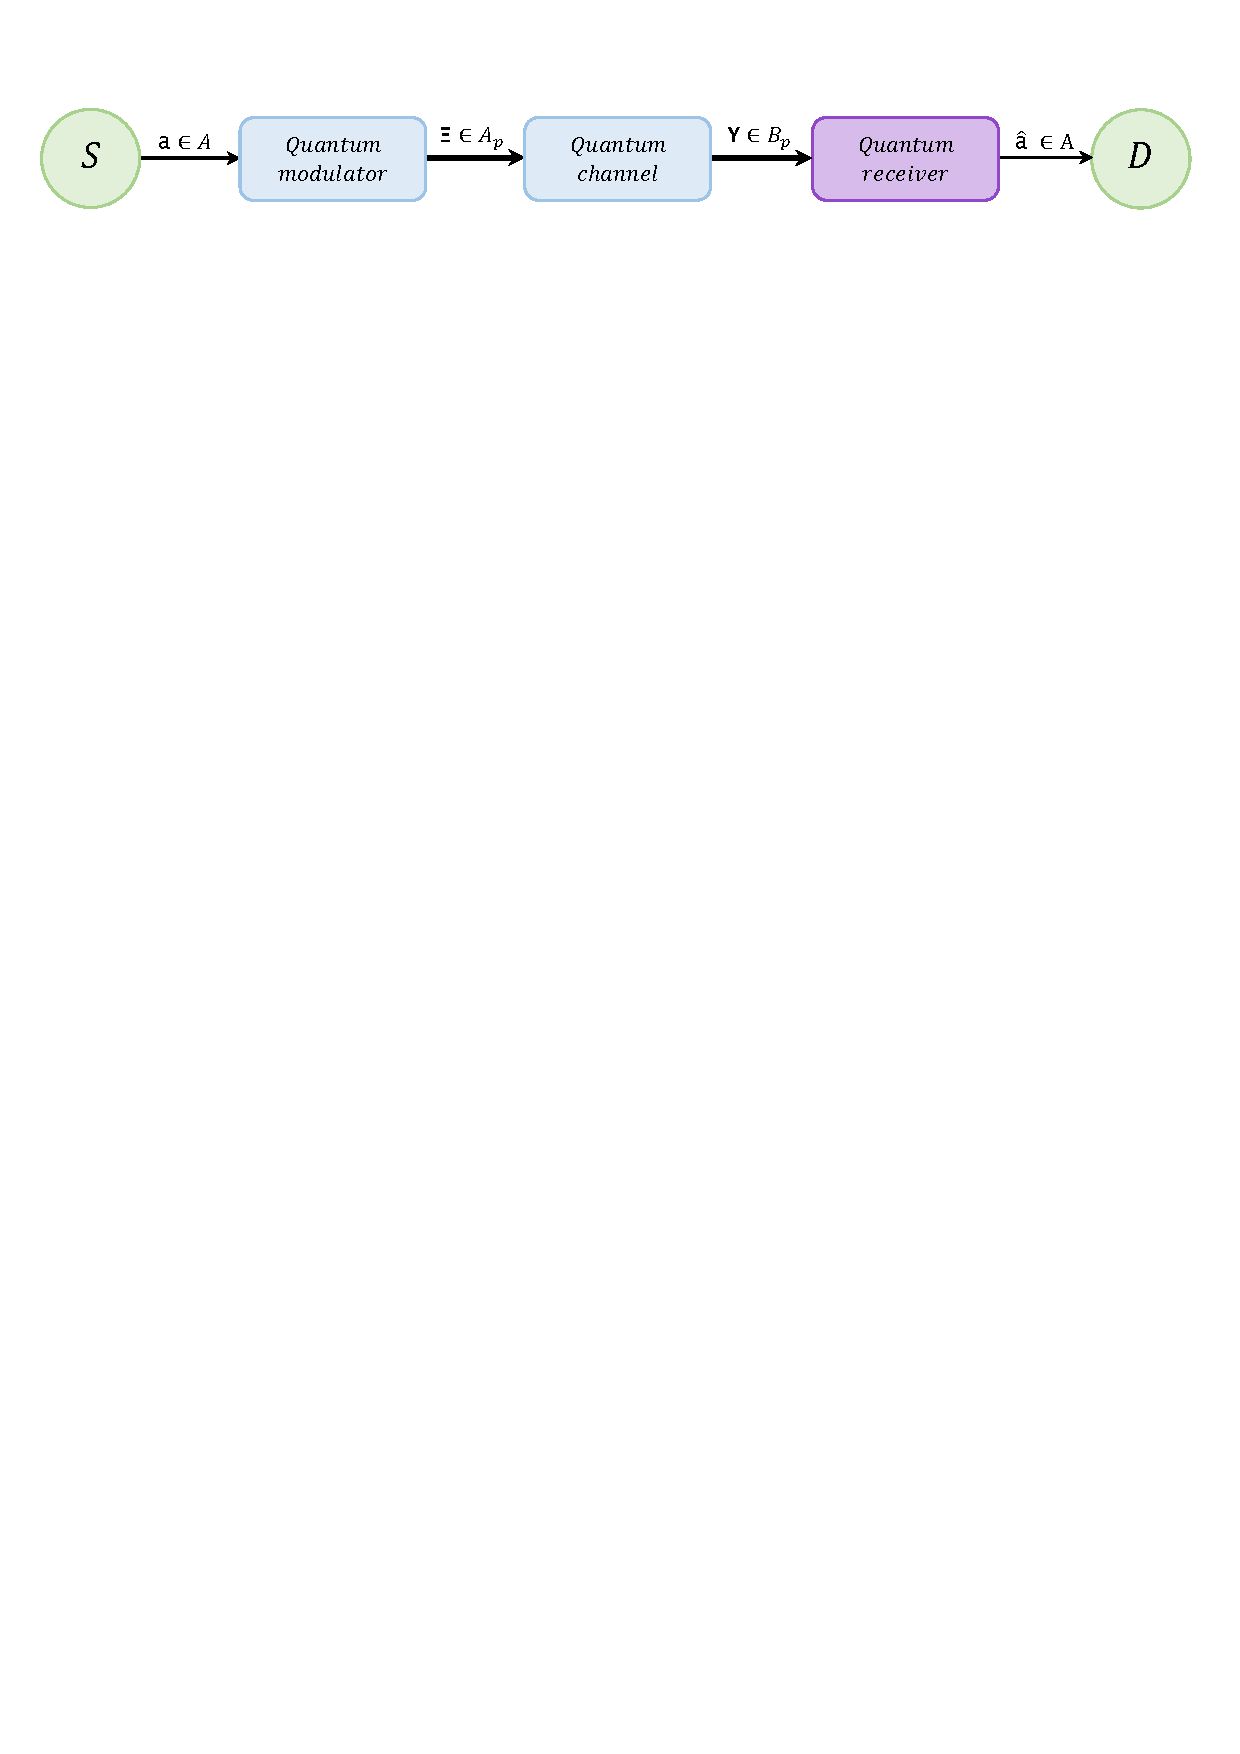
\includegraphics[width=0.8\textwidth]{fig3.1.pdf}
            \caption{MDEP for PACS QOOK with: $k=0,1,2,3$; $\bar{n}=10^{-2}$; $p_0=p_1=1/2$}
            \label{fig:3.1}
        \end{center}
    \end{figure}
    The MDEP of a quantum OOK system with PACS in function of $n_p$ is represented in the figure
    \ref{fig:3.1}, where in the x-axis there are the mean number of photon $n_p$ in the state 
    $\Operator{\varXi}_1$ (which corresponds to the mean number of photon in the whole system) and in the 
    y-axes there are the MDEP ($P_e$). The plot was obtained for equiprobable symbols and 
    mean number of thermal photons $\bar{n}=10^{-2}$.  
    The argument of the trace norm $\norm{\cdot}_1$ in the Helstrom bound 
    \ref{eq:HelstromBound}, is an operator in an infinite dimensional Hilbert space; for the 
    simulation, it has been approximated in $N=30$ dimension.
    We can observe that the photon addition improves significantly the performance in terms
    of error probability. Incrasing the value of the parameter $k$ the MDEP of the system 
    transate; the error probability, for the same energy-level, is lower if $k$ is bigger.
    We can notice too that the graphs do not start all from $0$. This is because the minimum
    mean number of photons in a photon added state is not always $0$ as it possible to see in 
    equation \ref{eq:min_np}.  

    \subsection{Quantum BPSK}
    It can be interesting to assess the effect of photon addition in a quantum BPSK system.
    The constellation is given, for a PACS BPSK, by:
    \begin{equation}\begin{split}
        \Operator{\varXi}_0 &=  \Operator{\varXi}_{\mathrm{th}} = \Operator{\varXi}_{\mathrm{th}}^{(k)}(-\mu)\\
        \Operator{\Xi}_1 &=  \Operator{\varXi}_{\mathrm{th}}^{(k)}(\mu).
    \end{split}\end{equation}
    %
    In absence of noise ($\bar{n}=0$), the MDEP is given by formula \ref{eq:HelstromBPure} where
    \begin{equation}
        \begin{split}
            \ket{\psi_0}&=\ket*{-\mu^{(k)}},\\
            \ket{\psi_1}&=\ket*{\mu^{(k)}}.
        \end{split}
    \end{equation}
    %
    The inner product is given, in closed form, by \cite{PACSDisc}:
    \begin{equation}
        \braket*{-\mu^{(k)}}{\mu^{(k)}} = \frac{L_k(\absolutevalue{\mu}^2)}{L_k(-\absolutevalue{\mu}^2)}
        e^{-2\absolutevalue{\mu}^2},
        \label{eq:innerp_nonNoise}
    \end{equation}
    where $L_k(x)$ is the Laguerre polynomial of parameter $k$, evaluate in $x$.
    \begin{figure}[t]
        \begin{subfigure}{0.5\textwidth}
            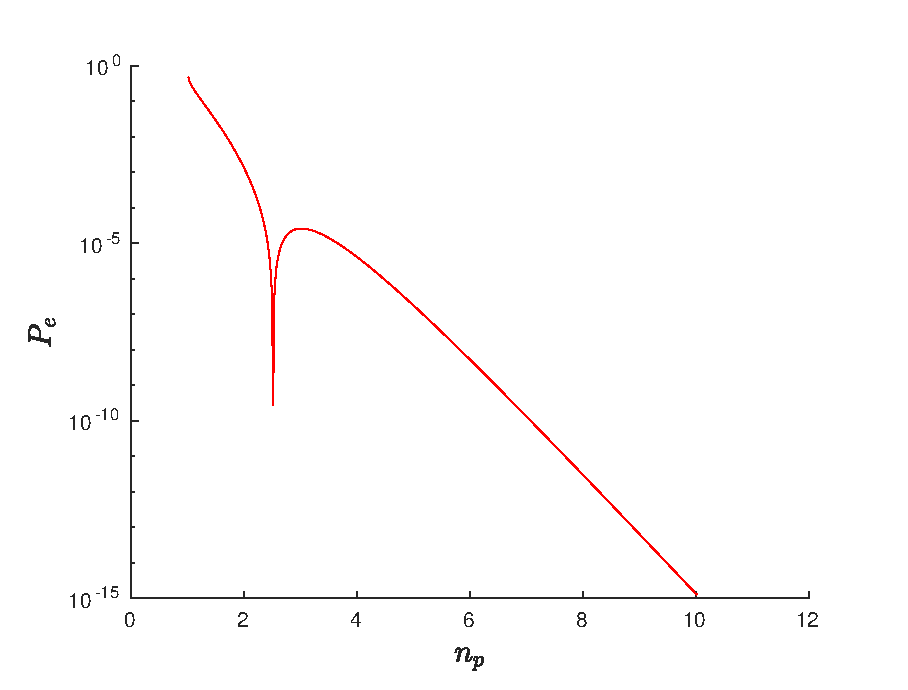
\includegraphics[width=\linewidth]{fig3.2a.eps}
            \caption{$k=1$}
        \end{subfigure}
        %\hspace*{fill}
        \begin{subfigure}{0.5\textwidth}
            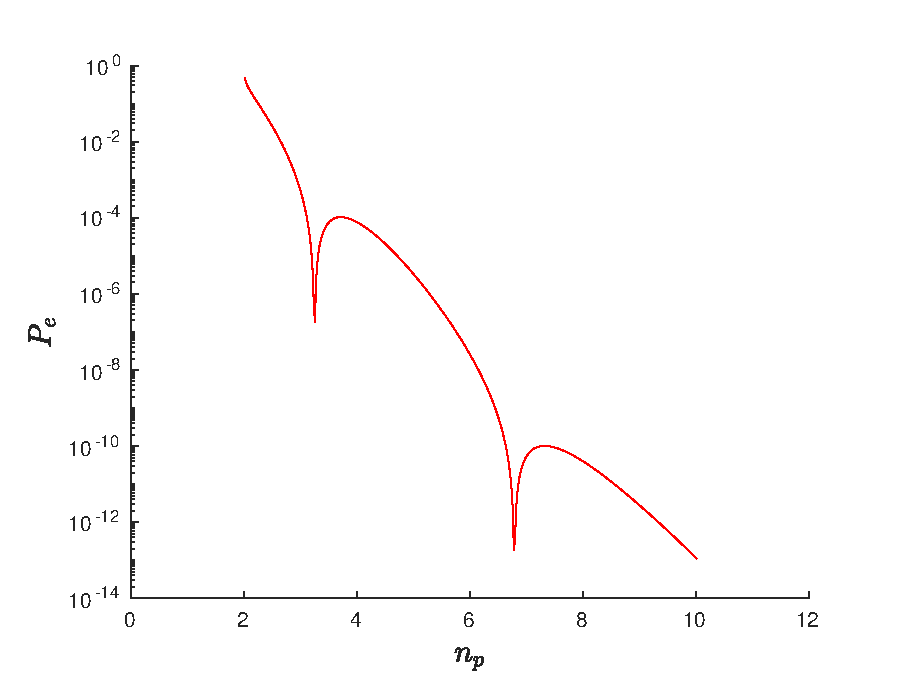
\includegraphics[width=\linewidth]{fig3.2b.eps}
            \caption{$k=2$}
        \end{subfigure}
        \caption{MDEP of quantum BPSK in absence of noise, $N=30$.}
        \label{fig:3.2}
    \end{figure}
    In figure \ref{fig:3.2} the MDEP in absence of noise, for QBPSK with PACS, is plotted for
    $k=1$ and for $k=2$, in function of $n_p$, with $N=30$. It can be noticed that exist $k$ zeros
    in the MDEP plot, where $k$ is the number of photon additions, that corresponds to the zeros
    of $L_k(\absolutevalue{\mu}^2)$ in equation \ref{eq:innerp_nonNoise}.
    The existence of these zeros is not really useful for the design of a quantum communication
    system because their selectivity factors are too high for a phisical implementation. It is, 
    nevertheless, possible to use that in order to evaluate the effect of the thermal noise.
    \begin{figure}[t]
        \begin{subfigure}{0.5\textwidth}
            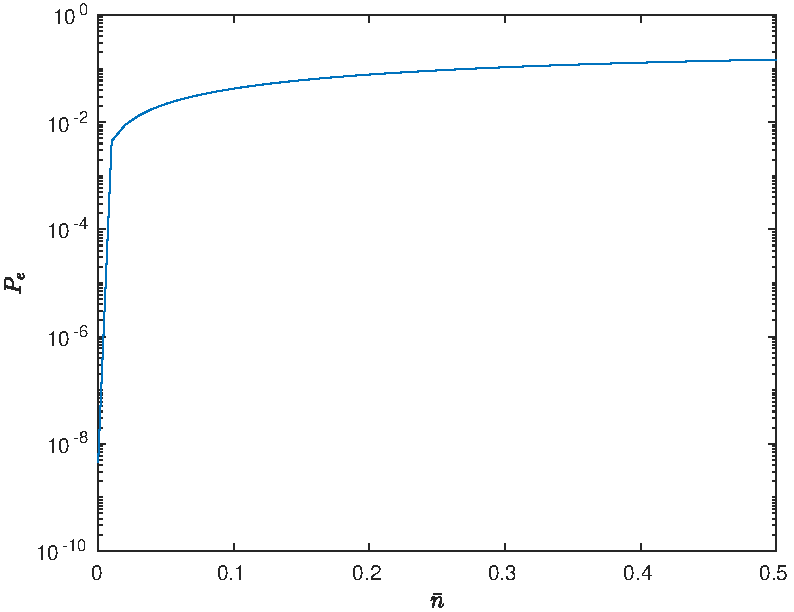
\includegraphics[width=\linewidth]{fig3.3a.pdf}
            \caption{$k=1$ \& $\mu = 0.54$}
        \end{subfigure}
        %\hspace*{fill}
        \begin{subfigure}{0.5\textwidth}
            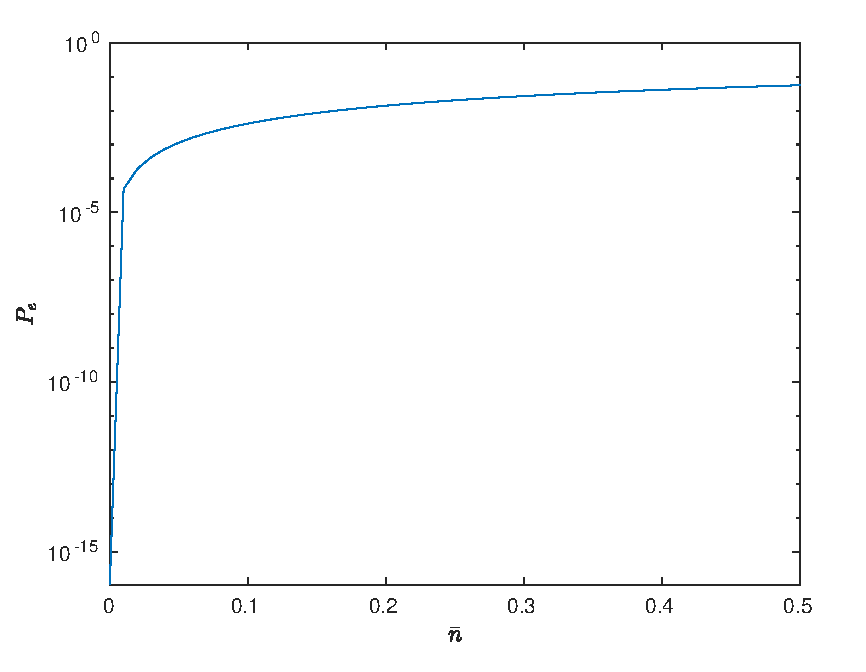
\includegraphics[width=\linewidth]{fig3.3b.pdf}
            \caption{$k=2$ \& $\mu = 1.58$}
        \end{subfigure}
        \caption{Thermal noise effect, in corrispondence of MDEP zeros ($N=40$).}
        \label{fig:3.3}
    \end{figure}
    In figure \ref{fig:3.3}, the sluggish performance due to the thermal noise is clear. The plot
    shows the trend of MDEP, for zeros value of $\mu$, in function of $\bar{n}$; the used approximation
    is $N=30$. The MDEP in presence of noise is given using the expression \ref{eq:HelstromBound}.
    We can shown using the formula \ref{eq:nbar} that $\bar{n}$ in a real cases in near to zero, the 
    plot show the general trend of the MDEP.

    \begin{figure}[t]
        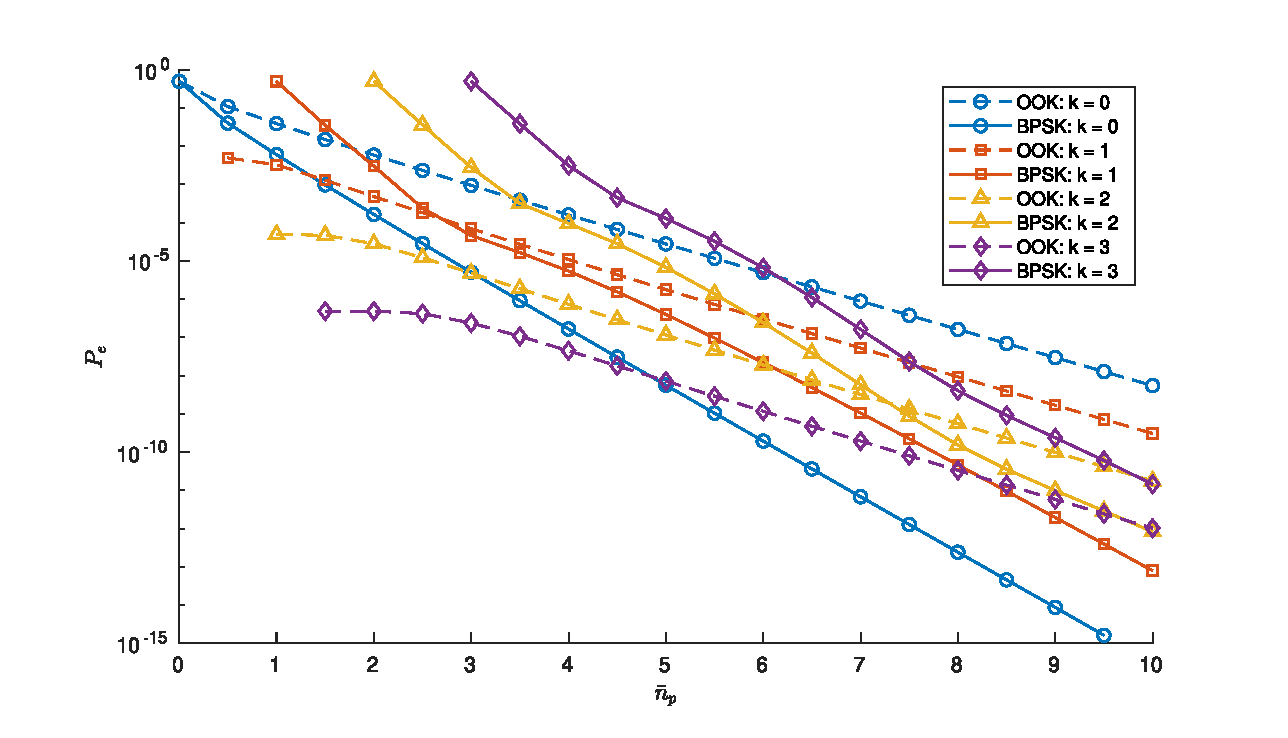
\includegraphics[width=1\textwidth]{fig3.4.eps}
        \caption{BPSK and OOK comparison. \\$N=45$, $\bar{n}=10^{-2}$, $p_0=p_1=1/2$}
        \label{fig:3.4}
    \end{figure}
    The comparison between a quantum OOK system and a quantum BPSK system is given in figure 
    \ref{fig:3.4}, in function of the mean number of photons in the system $\bar{E}$:
    \begin{equation*}
        \bar{E}=\frac{1}{2} \left(n_{p0}+n_{p1}\right),
    \end{equation*}
    where $n_{pi}$ is the mean number of photons in the state $\Operator{\varXi}_i$.
    The parameter $\bar{E}$ is equal to $n_p/2$ for the OOK system and the average of the $n_p$ for 
    each state for the BPSK system.
    The plots are given with $\bar{n}= 10^{-2}$, $N=45$ and equiprobable symbols.
    The obtained result is really intresting: the quantum BPSK has a sluggish performance due two 
    the photon addition process. At an equal level of energy $\bar{E}$, for PACS systems, it is
    possible to find an OOK configuration that maximizes the performance.
    
    %\section{Quantum communication systems with squeezed states}
    In this section we assess the effect of squeezing on the performance in absence of photon 
    addition and thermal noise. The representation of squeezed states are given in \ref{squeezedStates}.
    As for PACS systems, it can be useful to define the mean 
    number of photon $n_p$ in a squeezed state, which is given by
    \begin{equation}
        n_p(\mu,r) = \absolutevalue{\mu}^2 + \left(\sinh{r}\right)^2;
    \end{equation}
    where $\mu$ is the amplitude of the starter coherent state and the squeezing factor
    is $\zeta = r e^{i\theta}$. The minimum value of $n_p$ is given by $n_p(0,r) = \sinh{r}^2$.

    \subsection{Quantum OOK}
    \begin{figure}[t]
        % This file was created by matlab2tikz.
%
%The latest updates can be retrieved from
%  http://www.mathworks.com/matlabcentral/fileexchange/22022-matlab2tikz-matlab2tikz
%where you can also make suggestions and rate matlab2tikz.
%
\definecolor{mycolor1}{rgb}{1.00000,0.00000,1.00000}%
\definecolor{mycolor2}{rgb}{0.00000,1.00000,1.00000}%
%
\begin{tikzpicture}

\begin{axis}[%
width=4.521in,
height=3.566in,
at={(0.758in,0.481in)},
scale only axis,
unbounded coords=jump,
xmin=0,
xmax=4,
xlabel style={font=\color{white!15!black}},
xlabel={$\bar{n}_p$},
ymode=log,
ymin=0.000952035382554339,
ymax=1,
yminorticks=true,
ylabel style={font=\color{white!15!black}},
ylabel={$P_e$},
axis background/.style={fill=white},
axis x line*=bottom,
axis y line*=left,
legend style={legend cell align=left, align=left, draw=white!15!black}
]
\addplot [color=red]
  table[row sep=crcr]{%
0	0.4996948239481\\
0.1	0.345757180805158\\
0.2	0.287121156846032\\
0.3	0.24545028417787\\
0.4	0.212911022589419\\
0.5	0.186364156125375\\
0.6	0.164146896047426\\
0.7	0.145241250969801\\
0.8	0.128963672155848\\
0.9	0.114827686582853\\
1	0.102469669846838\\
1.1	0.0916098861017105\\
1.2	0.0820267587705495\\
1.3	0.0735410565066186\\
1.4	0.0660058406114885\\
1.5	0.059298707245483\\
1.6	0.0533166878041113\\
1.7	0.0479720733113359\\
1.8	0.0431899288477867\\
1.9	0.0389056427143193\\
2	0.0350630885593494\\
2.1	0.0316133642448069\\
2.2	0.0285137165123738\\
2.3	0.0257264385174695\\
2.4	0.0232184857173818\\
2.5	0.0209604826478608\\
2.6	0.018926505879439\\
2.7	0.0170934733750665\\
2.8	0.015440858978732\\
2.9	0.0139503375508124\\
3	0.0126055969522582\\
3.1	0.0113920033292345\\
3.2	0.0102964976303588\\
3.3	0.00930735236679731\\
3.4	0.00841405465378259\\
3.5	0.00760715856948718\\
3.6	0.0068781912376874\\
3.7	0.00621951875544752\\
3.8	0.00562428411547444\\
3.9	0.00508630643116037\\
4	0.00460003679294951\\
};
\addlegendentry{r = 0}

\addplot [color=red, only marks, mark=o, mark options={solid, red}]
  table[row sep=crcr]{%
0	0.4996948239481\\
};
\addlegendentry{r = 0.01}

\addplot [color=red, only marks, mark=o, mark options={solid, red}]
  table[row sep=crcr]{%
0.5	0.4996948239481\\
};
\addlegendentry{r = 0.1}

\addplot [color=red, only marks, mark=o, mark options={solid, red}]
  table[row sep=crcr]{%
1	0.4996948239481\\
};
\addlegendentry{r = 0.2}

\addplot [color=red, only marks, mark=o, mark options={solid, red}]
  table[row sep=crcr]{%
1.5	0.4996948239481\\
};
\addlegendentry{r = 0.5}

\addplot [color=red, only marks, mark=o, mark options={solid, red}, forget plot]
  table[row sep=crcr]{%
2	0.4996948239481\\
};
\addplot [color=red, only marks, mark=o, mark options={solid, red}, forget plot]
  table[row sep=crcr]{%
2.5	0.4996948239481\\
};
\addplot [color=red, only marks, mark=o, mark options={solid, red}, forget plot]
  table[row sep=crcr]{%
3	0.4996948239481\\
};
\addplot [color=red, only marks, mark=o, mark options={solid, red}, forget plot]
  table[row sep=crcr]{%
3.5	0.4996948239481\\
};
\addplot [color=red, only marks, mark=o, mark options={solid, red}, forget plot]
  table[row sep=crcr]{%
4	0.4996948239481\\
};
\addplot [color=green, forget plot]
  table[row sep=crcr]{%
0	nan\\
0.1	0.345064018736899\\
0.2	0.286187372245113\\
0.3	0.244381641821762\\
0.4	0.211763047105019\\
0.5	0.185173064834948\\
0.6	0.162937642185644\\
0.7	0.144031757964237\\
0.8	0.127767275529543\\
0.9	0.113654069132882\\
1	0.10132632364131\\
1.1	0.0905020842185692\\
1.2	0.0809582894225724\\
1.3	0.0725146416016301\\
1.4	0.0650232396075375\\
1.5	0.0583608166530484\\
1.6	0.0524237219713765\\
1.7	0.0471239463376132\\
1.8	0.0423861549024593\\
1.9	0.0381452869835203\\
2	0.0343451214923461\\
2.1	0.03093645129925\\
2.2	0.0278764546767297\\
2.3	0.0251273768898007\\
2.4	0.0226560519684494\\
2.5	0.0204330668185038\\
2.6	0.0184324797606132\\
2.7	0.0166312087814519\\
2.8	0.0150087416267342\\
2.9	0.0135467790137929\\
3	0.0122290428253946\\
3.1	0.0110409651304977\\
3.2	0.00996948449447915\\
3.3	0.00900297076544082\\
3.4	0.00813092412607835\\
3.5	0.00734397700992612\\
3.6	0.00663371401765406\\
3.7	0.00599257358816813\\
3.8	0.0054137275868128\\
3.9	0.00489107971825575\\
4	0.004419112867945\\
};
\addplot [color=green, only marks, mark=square, mark options={solid, green}, forget plot]
  table[row sep=crcr]{%
0	nan\\
};
\addplot [color=green, only marks, mark=square, mark options={solid, green}, forget plot]
  table[row sep=crcr]{%
0.5	nan\\
};
\addplot [color=green, only marks, mark=square, mark options={solid, green}, forget plot]
  table[row sep=crcr]{%
1	nan\\
};
\addplot [color=green, only marks, mark=square, mark options={solid, green}, forget plot]
  table[row sep=crcr]{%
1.5	nan\\
};
\addplot [color=green, only marks, mark=square, mark options={solid, green}, forget plot]
  table[row sep=crcr]{%
2	nan\\
};
\addplot [color=green, only marks, mark=square, mark options={solid, green}, forget plot]
  table[row sep=crcr]{%
2.5	nan\\
};
\addplot [color=green, only marks, mark=square, mark options={solid, green}, forget plot]
  table[row sep=crcr]{%
3	nan\\
};
\addplot [color=green, only marks, mark=square, mark options={solid, green}, forget plot]
  table[row sep=crcr]{%
3.5	nan\\
};
\addplot [color=green, only marks, mark=square, mark options={solid, green}, forget plot]
  table[row sep=crcr]{%
4	nan\\
};
\addplot [color=blue, forget plot]
  table[row sep=crcr]{%
0	nan\\
0.1	0.342911242050718\\
0.2	0.28058961140917\\
0.3	0.237013615624501\\
0.4	0.203362627785208\\
0.5	0.176172423921015\\
0.6	0.153621129473415\\
0.7	0.134598552001024\\
0.8	0.118361111210907\\
0.9	0.104380130690808\\
1	0.0922620419252684\\
1.1	0.0817039223529157\\
1.2	0.0724666945589215\\
1.3	0.0643575588674198\\
1.4	0.0572190562504042\\
1.5	0.0509203137421171\\
1.6	0.0453515615989874\\
1.7	0.0404200410126793\\
1.8	0.036046499652801\\
1.9	0.0321631768342768\\
2	0.0287114380592102\\
2.1	0.0256404630750137\\
2.2	0.0229061115233933\\
2.3	0.0204696999940017\\
2.4	0.0182975075201901\\
2.5	0.0163597742310368\\
2.6	0.0146303978697211\\
2.7	0.0130863360990972\\
2.8	0.0117072108830385\\
2.9	0.0104750164931909\\
3	0.00937374288410803\\
3.1	0.00838926633942438\\
3.2	0.00750897215726454\\
3.3	0.00672168429436226\\
3.4	0.00601744615112698\\
3.5	0.00538739392489546\\
3.6	0.004823640184214\\
3.7	0.0043191402885786\\
3.8	0.00386760371936712\\
3.9	0.00346344111948527\\
4	0.00310164723719591\\
};
\addplot [color=blue, only marks, mark=triangle, mark options={solid, blue}, forget plot]
  table[row sep=crcr]{%
0	nan\\
};
\addplot [color=blue, only marks, mark=triangle, mark options={solid, blue}, forget plot]
  table[row sep=crcr]{%
0.5	nan\\
};
\addplot [color=blue, only marks, mark=triangle, mark options={solid, blue}, forget plot]
  table[row sep=crcr]{%
1	nan\\
};
\addplot [color=blue, only marks, mark=triangle, mark options={solid, blue}, forget plot]
  table[row sep=crcr]{%
1.5	nan\\
};
\addplot [color=blue, only marks, mark=triangle, mark options={solid, blue}, forget plot]
  table[row sep=crcr]{%
2	nan\\
};
\addplot [color=blue, only marks, mark=triangle, mark options={solid, blue}, forget plot]
  table[row sep=crcr]{%
2.5	nan\\
};
\addplot [color=blue, only marks, mark=triangle, mark options={solid, blue}, forget plot]
  table[row sep=crcr]{%
3	nan\\
};
\addplot [color=blue, only marks, mark=triangle, mark options={solid, blue}, forget plot]
  table[row sep=crcr]{%
3.5	nan\\
};
\addplot [color=blue, only marks, mark=triangle, mark options={solid, blue}, forget plot]
  table[row sep=crcr]{%
4	nan\\
};
\addplot [color=mycolor1, forget plot]
  table[row sep=crcr]{%
0	nan\\
0.1	0.352483179556453\\
0.2	0.282015320063401\\
0.3	0.234732372951055\\
0.4	0.198938618050338\\
0.5	0.170422220223627\\
0.6	0.147047605722407\\
0.7	0.12753619551938\\
0.8	0.111045202459609\\
0.9	0.0969796510639878\\
1	0.0849000679635937\\
1.1	0.0744706800960189\\
1.2	0.0654275840690521\\
1.3	0.0575597358535224\\
1.4	0.0506950380305154\\
1.5	0.0446916628730589\\
1.6	0.0394311481668558\\
1.7	0.0348141620942864\\
1.8	0.030756195940998\\
1.9	0.0271853117419146\\
2	0.0240397830099432\\
2.1	0.0212665456031397\\
2.2	0.0188196302835341\\
2.3	0.0166592253798481\\
2.4	0.0147506425523341\\
2.5	0.0130637022853067\\
2.6	0.0115720329348848\\
2.7	0.0102524759571693\\
2.8	0.00908478476977853\\
2.9	0.00805119723079872\\
3	0.00713606551874252\\
3.1	0.00632562120224001\\
3.2	0.00560774441838796\\
3.3	0.00497174792321697\\
3.4	0.00440820528309399\\
3.5	0.00390878880218942\\
3.6	0.00346615989599225\\
3.7	0.00307380367294957\\
3.8	0.00272598065309104\\
3.9	0.00241761535472995\\
4	0.00214420611137395\\
};
\addplot [color=mycolor1, only marks, mark=diamond, mark options={solid, mycolor1}, forget plot]
  table[row sep=crcr]{%
0	nan\\
};
\addplot [color=mycolor1, only marks, mark=diamond, mark options={solid, mycolor1}, forget plot]
  table[row sep=crcr]{%
0.5	nan\\
};
\addplot [color=mycolor1, only marks, mark=diamond, mark options={solid, mycolor1}, forget plot]
  table[row sep=crcr]{%
1	nan\\
};
\addplot [color=mycolor1, only marks, mark=diamond, mark options={solid, mycolor1}, forget plot]
  table[row sep=crcr]{%
1.5	nan\\
};
\addplot [color=mycolor1, only marks, mark=diamond, mark options={solid, mycolor1}, forget plot]
  table[row sep=crcr]{%
2	nan\\
};
\addplot [color=mycolor1, only marks, mark=diamond, mark options={solid, mycolor1}, forget plot]
  table[row sep=crcr]{%
2.5	nan\\
};
\addplot [color=mycolor1, only marks, mark=diamond, mark options={solid, mycolor1}, forget plot]
  table[row sep=crcr]{%
3	nan\\
};
\addplot [color=mycolor1, only marks, mark=diamond, mark options={solid, mycolor1}, forget plot]
  table[row sep=crcr]{%
3.5	nan\\
};
\addplot [color=mycolor1, only marks, mark=diamond, mark options={solid, mycolor1}, forget plot]
  table[row sep=crcr]{%
4	nan\\
};
\addplot [color=mycolor2, forget plot]
  table[row sep=crcr]{%
0	nan\\
0.1	nan\\
0.2	nan\\
0.3	0.306786766345818\\
0.4	0.242590630097618\\
0.5	0.197918895572083\\
0.6	0.164073400870317\\
0.7	0.137366478836737\\
0.8	0.115784377573039\\
0.9	0.0980699796818669\\
1	0.0833714751942309\\
1.1	0.0710774586522101\\
1.2	0.0607327341300646\\
1.3	0.0519875094320926\\
1.4	0.0445671089158063\\
1.5	0.0382519606700177\\
1.6	0.0328646519862905\\
1.7	0.0282596802292375\\
1.8	0.0243169681921276\\
1.9	0.0209367128708955\\
2	0.0180353163612855\\
2.1	0.0155426264094213\\
2.2	0.013399252202812\\
2.3	0.0115550198413198\\
2.4	0.00996724028084983\\
2.5	0.00859955485624092\\
2.6	0.00742097560285826\\
2.7	0.00640497624240516\\
2.8	0.0055288612502285\\
2.9	0.0047731718879836\\
3	0.00412119408203854\\
3.1	0.00355860194225149\\
3.2	0.00307303906910844\\
3.3	0.00265391333494414\\
3.4	0.00229208259247371\\
3.5	0.00197968020442113\\
3.6	0.00170993158525734\\
3.7	0.00147699358221837\\
3.8	0.00127582696954853\\
3.9	0.00110208961226266\\
4	0.000952035382554339\\
};
\addplot [color=mycolor2, only marks, mark=star, mark options={solid, mycolor2}, forget plot]
  table[row sep=crcr]{%
0	nan\\
};
\addplot [color=mycolor2, only marks, mark=star, mark options={solid, mycolor2}, forget plot]
  table[row sep=crcr]{%
0.5	nan\\
};
\addplot [color=mycolor2, only marks, mark=star, mark options={solid, mycolor2}, forget plot]
  table[row sep=crcr]{%
1	nan\\
};
\addplot [color=mycolor2, only marks, mark=star, mark options={solid, mycolor2}, forget plot]
  table[row sep=crcr]{%
1.5	nan\\
};
\addplot [color=mycolor2, only marks, mark=star, mark options={solid, mycolor2}, forget plot]
  table[row sep=crcr]{%
2	nan\\
};
\addplot [color=mycolor2, only marks, mark=star, mark options={solid, mycolor2}, forget plot]
  table[row sep=crcr]{%
2.5	nan\\
};
\addplot [color=mycolor2, only marks, mark=star, mark options={solid, mycolor2}, forget plot]
  table[row sep=crcr]{%
3	nan\\
};
\addplot [color=mycolor2, only marks, mark=star, mark options={solid, mycolor2}, forget plot]
  table[row sep=crcr]{%
3.5	nan\\
};
\addplot [color=mycolor2, only marks, mark=star, mark options={solid, mycolor2}, forget plot]
  table[row sep=crcr]{%
4	nan\\
};
\end{axis}

\begin{axis}[%
width=5.833in,
height=4.375in,
at={(0in,0in)},
scale only axis,
xmin=0,
xmax=1,
ymin=0,
ymax=1,
axis line style={draw=none},
ticks=none,
axis x line*=bottom,
axis y line*=left
]
\end{axis}
\end{tikzpicture}%
        \caption{MDEP of OOK squeezed states system as function of $\bar{n}_p$ without thermal 
        noise, $N=45$, $\theta=\pi$ and equiprobable symbols.}
        \label{fig:OOK_SS}
    \end{figure}
    A quantum OOK system with squeezed states is a system with the following constellation
    \begin{subequations}
        \begin{align}
            \Operator{\varXi}_0 &= \Operator{\varXi}(0,0)\\
            \Operator{\varXi}_1 &= \Operator{\varXi}(\mu,\zeta)
        \end{align}
    \end{subequations}
    where $\Operator{\varXi}_{\mathrm{th}}(\mu,\zeta)$ is the squeezed state with amplitude $\mu$
    and squeezing parameter $\zeta$.

    The MDEP as function of $\bar{n}_p$,
    i.e the mean number of photon in the system,  is plotted in figure \ref{fig:OOK_SS} with:
    $\theta=\pi$, $N=45$, equiprobable symbols and $\bar{n}=0$.
    It can be noticed that the optimal configuration of $r$ depends on the energy in the 
    system. For low energy levels the squeezing has not a positive effect.
    \subsection{Quantum BPSK}
    The effect of the squeezing in a BPSK system is similar to that in the OOK. The constellation
    of this type of system is given by
    \begin{subequations}
        \begin{align}
            \Operator{\varXi}_0 &= \Operator{\varXi}(-\mu,\zeta)\\
            \Operator{\varXi}_1 &= \Operator{\varXi}(\mu,\zeta).
        \end{align}
    \end{subequations}
    Figure \ref{fig:3.5} shows the MDEP of the system as function of $\bar{n}_p$
    with $\theta=\pi$, $N=45$, equiprobable symbols and $\bar{n}=0$.

    \begin{figure}[t]
        \begin{center}
            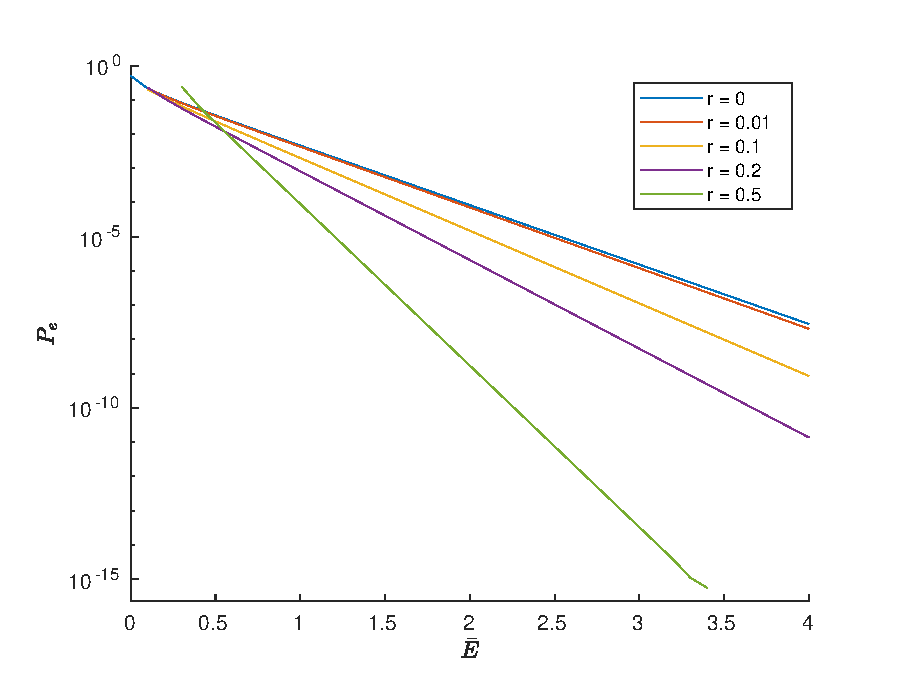
\includegraphics[width=0.8\textwidth]{fig3.5.eps}
            \caption{MDEP of squeezed state BPSK system as function of $\bar{n}_p$. 
                $N=30$, $\bar{n}=0$, $\theta=\pi$, $p_0=p_1=1/2$}
            \label{fig:3.5}
        \end{center}     
    \end{figure}
    \section{Quantum communication systems with PASSs}
    The use of squeezed states instead of coherent states allows us to overcome the limits
    of precedent systems. The representation of a noisy squeezed state is given in 
    \ref{squeezedStates}. The correspondend photon added state is obtained using the equation
    \ref{eq:photonAddedState} and it is described in \ref{PASSs}. This section discusses the advantages of using PASSs 
    in quantum OOK and BPSK systems.

    The MDEP for PASSs systems is found again with the Helstrom bound \ref{eq:HelstromBound}.
    As for the other systems, it is useful to define the mean number of photons $n_p$ for noisy 
    photon added squeezed states, that is given by:
    \begin{equation}
        n_p(\mu,\zeta,\bar{n}) = \frac{N_{k+1}(\mu,\zeta,\bar{n})}{N_k(\mu,\zeta,\bar{n})}-1,
        \label{eq:np_PASS}
    \end{equation}
    where
    \begin{equation}
        \begin{split}
            N_k(\mu,\zeta,\bar{n}) &= \tr{(\Operator{A}^\dagger)^k \Operator{\varXi}_{\mathrm{th}}(\mu,\zeta) \Operator{A}^k}\\
                                    &= \tr{(\Operator{A}^\dagger)^k \Operator{D}_\mu \Operator{S}_\zeta \Operator{\varXi}_{\mathrm{th}}
                                    \Operator{S}_\zeta^\dagger \Operator{D}_\mu^\dagger \Operator{A}^k}.
        \end{split}
    \end{equation}

    \subsection{Quantum OOK}
        The constellation of a quantum OOK system with noisy PASS, is given by:
        \begin{subequations}
            \begin{align}
                \Operator{\varXi}_0 &= \Operator{\varXi}_{\mathrm{th}}^{(0)}(0,0)\\
                \Operator{\varXi}_1 &= \Operator{\varXi}_{\mathrm{th}}^{(k)}(\mu,\zeta).
            \end{align}
        \end{subequations}
        In figure \ref{fig:3.6}, the MDEP of a quantum OOK noisy PASS system is plotted in function
        of the mean number of photon $\bar{n}_p$ in the system. For the simulation are used $N=30$, $\bar{n}=10^{-2}$, $\theta=\pi$ and
        equiprobable symbols.
        It can be noticed that the photon addition significantly improves the performance of the system,
        at least for the plotted energy level.

    \paragraph{Quantum BPSK}
        Similary to the PACS BPSK, the constellation of PASS BPSK is given by:
        \begin{subequations}
            \begin{align}
                \Operator{\varXi}_0 &= \Operator{\varXi}_{\mathrm{th}}^{(k)}(-\mu,\zeta)\\
                \Operator{\varXi}_1 &= \Operator{\varXi}_{\mathrm{th}}^{(k)}(\mu,\zeta).
            \end{align}
        \end{subequations}
        
        The figure \ref{fig:3.7} shows the effects of the photon addition in a quantum BPSK
        system, in terms of the mean photon number in the system $\bar{n}_p$, given by the average of 
        the mean photon number $n_p$ of $\Operator{\varXi}_0$ and $\Operator{\varXi}_1$. The parameters used
        for the simulation are $N=40$, $\bar{n}=10^{-2}$, $\theta=\pi$ and equiprobable symbols.
        As in PACS case, it is evident that the photon addition, in a BPSK system, has not
        the positive effect that has in an OOK system.
        
        \begin{figure}[t]
            \begin{center}
                %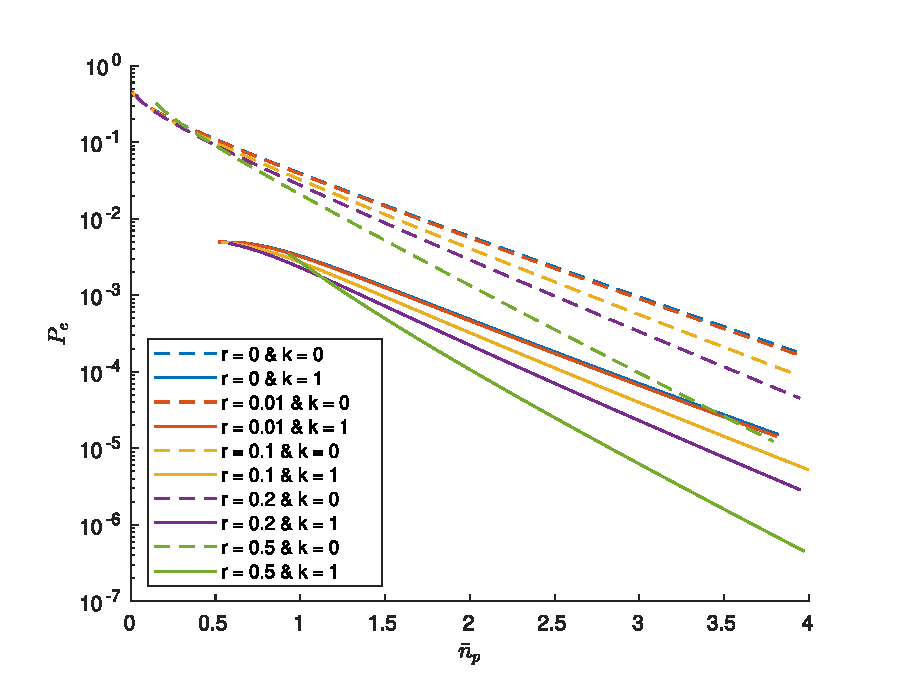
\includegraphics[width=0.8\textwidth]{fig3.6.eps}
                % This file was created by matlab2tikz.
%
%The latest updates can be retrieved from
%  http://www.mathworks.com/matlabcentral/fileexchange/22022-matlab2tikz-matlab2tikz
%where you can also make suggestions and rate matlab2tikz.
%
\definecolor{mycolor1}{rgb}{0.00000,0.44706,0.74118}%
\definecolor{mycolor2}{rgb}{0.85098,0.32549,0.09804}%
\definecolor{mycolor3}{rgb}{0.92941,0.69020,0.12941}%
\definecolor{mycolor4}{rgb}{0.49020,0.18039,0.56078}%
\definecolor{mycolor5}{rgb}{0.46667,0.67451,0.18824}%
%
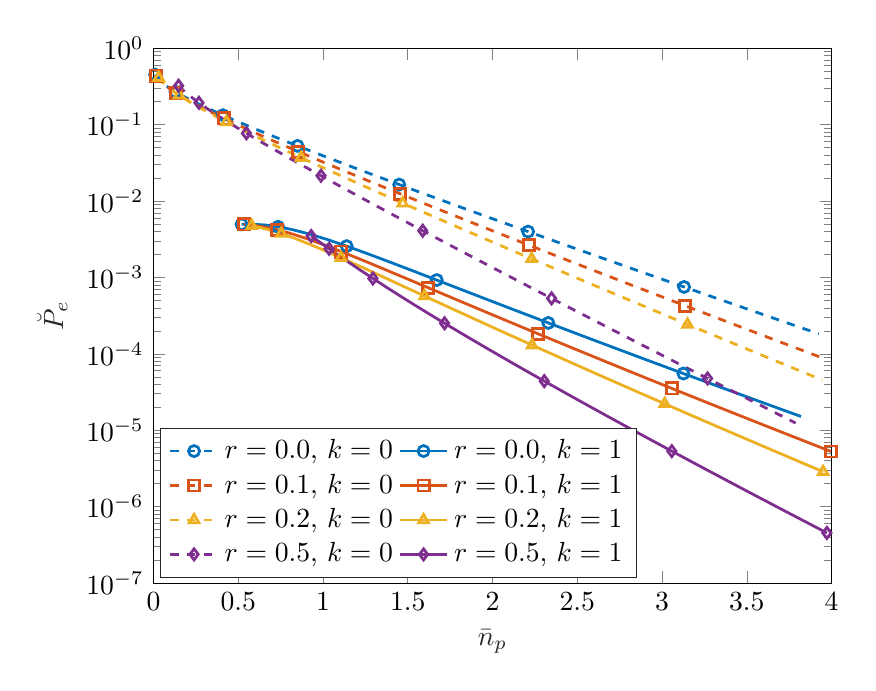
\begin{tikzpicture}

\begin{axis}[%
width=4.521in*0.75,
height=3.566in*0.75,
at={(0.758in,0.481in)},
scale only axis,
xmin=0,
xmax=4,
xlabel style={font=\color{white!15!black}},
xlabel={$\bar{n}_p$},
ymode=log,
ymin=1e-07,
ymax=1,
yminorticks=true,
ylabel style={font=\color{white!15!black}},
ylabel={$\breve{P}_e$},
axis background/.style={fill=white},
%axis x line*=bottom,
%axis y line*=left,
legend style={at={(0.01,0.01)}, anchor=south west, legend cell align=left, align=left, draw=white!15!black, legend columns=2}
]
\addplot [color=mycolor1, dashed, line width=1.0pt, mark=o, mark options={solid, mycolor1}, mark repeat={4}]
  table[row sep=crcr]{%
%0.0100000000010203	0.5\\
0.0100000000005099	0.451090572691058\\
0.0250000000005101	0.402886691283792\\
0.0500000000005101	0.356065452094155\\
0.08500000000051	0.311248795396144\\
0.13000000000051	0.268980151318818\\
0.18500000000051	0.229705791588748\\
0.25000000000051	0.193761885698297\\
0.32500000000051	0.161367836859558\\
0.41000000000051	0.132626017381623\\
0.50500000000051	0.107527572164159\\
0.61000000000051	0.0859635483991091\\
0.72500000000051	0.0677402706067526\\
0.850000000000511	0.0525976380078704\\
0.98500000000051	0.0402288938163128\\
1.13000000000051	0.030300412747497\\
1.28500000000051	0.0224701735043473\\
1.45000000000051	0.0164038154402497\\
1.62500000000051	0.0117874985937506\\
1.81000000000051	0.00833715723539569\\
2.00500000000051	0.00580411358757593\\
2.21000000000051	0.00397735316445369\\
2.42500000000051	0.00268301603344667\\
2.65000000000051	0.00178180465531275\\
2.88500000000051	0.00116504474732931\\
3.13000000000051	0.000750076554437373\\
3.38500000000051	0.000475529564681665\\
3.65000000000051	0.000296878649024612\\
3.92500000000051	0.000182524960914532\\
};
\addlegendentry{$r = 0.0$, $k = 0$}

\addplot [color=mycolor1, line width=1.0pt, mark=o, mark options={solid, mycolor1}, mark repeat={4}]
  table[row sep=crcr]{%
%1.02000000000307	0.00495049504950945\\
0.519950970393687	0.00495049504951145\\
0.549238056382468	0.00495049384760837\\
0.596318098365133	0.00494513949975245\\
0.659059689574124	0.00485212464085472\\
0.735198210318913	0.00459825907392819\\
0.822700461899245	0.00420399327465371\\
0.919966333468088	0.00369559902026673\\
1.02587839224384	0.00312976798911424\\
1.13975229329811	0.00256690084404709\\
1.26124327363325	0.00204996332234814\\
1.39024719180321	0.00160098998755381\\
1.52681572702182	0.00122639811266967\\
1.67109195414956	0.000923250889520943\\
1.8232653201361	0.000683888328226578\\
1.98354224079897	0.000498830625317581\\
2.15212812011347	0.000358440774981539\\
2.32921719287323	0.000253800056086939\\
2.51498745769556	0.000177110101371558\\
2.70959877008803	0.000121819045365512\\
2.91319279840464	8.25922216302066e-05\\
3.1258940040236	5.52004961243968e-05\\
3.34781112191599	3.63708050424849e-05\\
3.57903882606496	2.36261622261202e-05\\
3.81965939805169	1.51315705133603e-05\\
};
\addlegendentry{$r = 0.0$, $k = 1$}

\addplot [color=mycolor2, dashed, line width=1.0pt, mark=square, mark options={solid, mycolor2}, mark repeat={4}]
  table[row sep=crcr]{%
%0.0202340453657284	0.464473627654879\\
0.0151170226828645	0.437604627349995\\
0.0301170226828643	0.392232608937378\\
0.0551170226828643	0.345350311735397\\
0.0901170226828644	0.299872457829165\\
0.135117022682864	0.256926510392587\\
0.190117022682864	0.217172327050335\\
0.255117022682864	0.181031813929761\\
0.330117022682864	0.148752335319914\\
0.415117022682864	0.120429087835948\\
0.510117022682864	0.0960200366887284\\
0.615117022682864	0.0753645347394633\\
0.730117022682865	0.0582063945825236\\
0.855117022682864	0.0442194749392917\\
0.990117022682864	0.033033747624904\\
1.13511702268286	0.0242600166699049\\
1.29011702268286	0.0175117313604393\\
1.45511702268286	0.012422724228866\\
1.63011702268287	0.0086601979591992\\
1.81511702268287	0.00593281764231124\\
2.01011702268286	0.00399425837705447\\
2.21511702268287	0.00264294241797458\\
2.43011702268287	0.00171892901031734\\
2.65511702268286	0.00109898195775715\\
2.89011702268287	0.000690756906602363\\
3.13511702268287	0.000426868293537996\\
3.39011702268287	0.000259369510946184\\
3.65511702268287	0.000154957633989594\\
3.93011702268287	9.10290546821124e-05\\
};
\addlegendentry{$r = 0.1$, $k = 0$}

\addplot [color=mycolor2, line width=1.0pt, mark=square, mark options={solid, mycolor2}, mark repeat={4}]
  table[row sep=crcr]{%
%1.05080244685835	0.00494855515487186\\
0.534305855441027	0.00493956193944328\\
0.560577815242343	0.00489125057574918\\
0.603010711176586	0.00476554057726364\\
0.659935286045382	0.00454063398198279\\
0.729573342297954	0.00420193412015313\\
0.810323033235768	0.00375582941028574\\
0.90091844851316	0.0032368659457353\\
1.00047082343265	0.00269516501446371\\
1.10843171757119	0.00217671120450486\\
1.22452096613732	0.00171213398444298\\
1.3486495574248	0.00131595523776701\\
1.4808530565899	0.00099074984674008\\
1.62124071752346	0.000731856527585784\\
1.76995971625628	0.000531006006724011\\
1.92717165481784	0.000378693077575321\\
2.09303809416422	0.000265572059704344\\
2.26771230591607	0.000183193116200464\\
2.45133509281032	0.000124323441114904\\
2.64403315014596	8.30191324586171e-05\\
2.8459189361002	5.45554227568412e-05\\
3.05709138017673	3.5284096614796e-05\\
3.27763700858953	2.24616790437393e-05\\
3.50763123129931	1.40753992720621e-05\\
3.74713964255157	8.68275836485299e-06\\
3.99621925419453	5.27284023565944e-06\\
};
\addlegendentry{$r = 0.1$, $k = 1$}

\addplot [color=mycolor3, dashed, line width=1.0pt, mark=triangle, mark options={solid, mycolor3}, mark repeat={4}]
  table[row sep=crcr]{%
%0.051346909637612	0.429393647208632\\
0.0306734548188061	0.411688903318411\\
0.045673454818806	0.373223243143298\\
0.070673454818806	0.329064496412081\\
0.105673454818806	0.284699966244283\\
0.150673454818806	0.242312311121901\\
0.205673454818806	0.20300894013495\\
0.270673454818806	0.167412745153845\\
0.345673454818806	0.135848539010154\\
0.430673454818806	0.108424113178776\\
0.525673454818806	0.085074901679797\\
0.630673454818806	0.0655975019569672\\
0.745673454818806	0.0496824127447445\\
0.870673454818806	0.0369476450892914\\
1.00567345481881	0.0269714468453113\\
1.15067345481881	0.0193219002119312\\
1.30567345481881	0.0135816008581836\\
1.47067345481881	0.00936630014651907\\
1.64567345481881	0.00633712474233589\\
1.83067345481881	0.00420668870569196\\
2.02567345481881	0.00273998478983489\\
2.23067345481881	0.00175130670345874\\
2.44567345481881	0.00109858125431284\\
2.67067345481881	0.000676400651179798\\
2.90567345481881	0.000408804118392059\\
3.15067345481881	0.000242545209768685\\
3.40567345481881	0.000141270680246663\\
3.67067345481881	8.07790992743973e-05\\
3.94567345481881	4.53451833415941e-05\\
};
\addlegendentry{$r = 0.2$, $k = 0$}

\addplot [color=mycolor3, line width=1.0pt, mark=triangle, mark options={solid, mycolor3}, mark repeat={4}]
  table[row sep=crcr]{%
%1.14443400452204	0.00479106599394818\\
0.579999501304023	0.00475077465542328\\
0.603041046327231	0.00463108156969505\\
0.640504199710634	0.00442827805532442\\
0.691224117225214	0.00413258381262105\\
0.753950466998375	0.00374355433932783\\
0.827545812383434	0.00327986823785392\\
0.911100241882687	0.00277718849843345\\
1.00396497754985	0.00227642511237597\\
1.10573089526536	0.0018115455221398\\
1.21618079241689	0.00140378131439783\\
1.33523645804668	0.0010619876604348\\
1.46291195118471	0.000785891546957074\\
1.5992772335824	0.000569691758631641\\
1.7444321745409	0.000404922413376918\\
1.89848917670023	0.000282385374672289\\
2.06156226583414	0.0001933054291125\\
2.23376070757581	0.000129931168492581\\
2.41518563437222	8.57733261649951e-05\\
2.60592858523409	5.56215786678416e-05\\
2.80607120496685	3.54369671975441e-05\\
3.01568560586141	2.21846003883308e-05\\
3.23483507482365	1.36482495925461e-05\\
3.46357493039391	8.25216498795411e-06\\
3.70195341365423	4.90393868035621e-06\\
3.9500125478046	2.86426889811731e-06\\
};
\addlegendentry{$r = 0.2$, $k = 1$}

\addplot [color=mycolor4, dashed, line width=1.0pt, mark=diamond, mark options={solid, mycolor4}, mark repeat={4}]
  table[row sep=crcr]{%
%0.286971123755774	0.330768077356153\\
0.148485561877887	0.321870897864741\\
0.163485561877887	0.2980861532608\\
0.188485561877887	0.265400945113278\\
0.223485561877887	0.229097440353421\\
0.268485561877887	0.192694408147652\\
0.323485561877887	0.158325364694675\\
0.388485561877887	0.127217381024676\\
0.463485561877887	0.0999991591056063\\
0.548485561877887	0.0768883603237902\\
0.643485561877887	0.0578110254090491\\
0.748485561877886	0.042489385074143\\
0.863485561877887	0.0305142243008485\\
0.988485561877887	0.0214056829491879\\
1.12348556187789	0.0146637973864988\\
1.26848556187789	0.0098079816862493\\
1.42348556187789	0.00640463929230534\\
1.58848556187789	0.00408314565752849\\
1.76348556187788	0.00254163692367282\\
1.94848556187788	0.00154491239086835\\
2.14348556187788	0.000917124936882341\\
2.34848556187788	0.000531801834133649\\
2.56348556187788	0.000301247165333363\\
2.78848556187787	0.000166721564607453\\
3.02348556187786	9.01545309603957e-05\\
3.26848556187785	4.76353769972571e-05\\
3.52348556187783	2.45938563666614e-05\\
3.78848556187779	1.24073309797912e-05\\
};
\addlegendentry{$r = 0.5$, $k = 0$}

\addplot [color=mycolor4, line width=1.0pt, mark=diamond, mark options={solid, mycolor4}, mark repeat={4}]
  table[row sep=crcr]{%
%1.85306548733767	0.00353641115520514\\
0.930796962701587	0.00348196426464287\\
0.943656157582369	0.00332231969133245\\
0.965295445105895	0.00306951882024781\\
0.995980641808412	0.00274452597887531\\
1.03601054788413	0.00237451347003192\\
1.08567365297189	0.0019883961081173\\
1.14521827738196	0.00161265536534688\\
1.21483826418498	0.00126811447852393\\
1.29467137765998	0.000968122366654389\\
1.38480564628563	0.000718538771233457\\
1.48528924260403	0.000519112688197765\\
1.59614083486364	0.000365447596944291\\
1.71735873922715	0.000250906556350627\\
1.84892823171401	0.000168117888699859\\
1.9908269892895	0.000109991365809137\\
2.14302891711736	7.02953013373975e-05\\
2.30550670737067	4.38998630067355e-05\\
2.47823346100084	2.67972348785284e-05\\
2.66118364860192	1.59921449159883e-05\\
2.85433362280369	9.33241343792357e-06\\
3.05766183728397	5.32614461246084e-06\\
3.27114888140597	2.97307164354166e-06\\
3.49477740479924	1.62328253511257e-06\\
3.7285319812022	8.66931754384126e-07\\
3.97239894341011	4.5286496330732e-07\\
};
\addlegendentry{$r = 0.5$, $k = 1$}
\end{axis}
\end{tikzpicture}%
                \caption{MDEP of noisy PASS quantum OOK system as function of $\bar{n}_p$.\\
                $N=30$, $\bar{n}=10^{-2}$, $\theta=\pi$ and $p_0=p_1=1/2$.}
                \label{fig:3.6}
            \end{center}
        \end{figure}
        \begin{figure}[t]
            \begin{center}
                %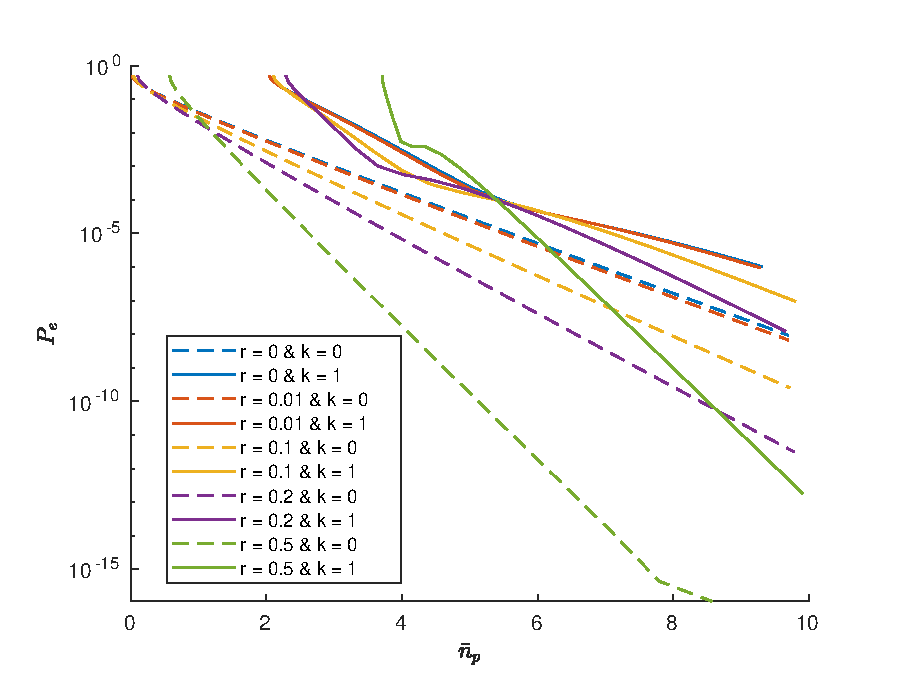
\includegraphics[width=0.8\textwidth]{fig3.7.eps}
                % This file was created by matlab2tikz.
%
%The latest updates can be retrieved from
%  http://www.mathworks.com/matlabcentral/fileexchange/22022-matlab2tikz-matlab2tikz
%where you can also make suggestions and rate matlab2tikz.
%
\definecolor{mycolor1}{rgb}{0.00000,0.44706,0.74118}%
\definecolor{mycolor2}{rgb}{0.85098,0.32549,0.09804}%
\definecolor{mycolor3}{rgb}{0.92941,0.69020,0.12941}%
\definecolor{mycolor4}{rgb}{0.49020,0.18039,0.56078}%
\definecolor{mycolor5}{rgb}{0.46667,0.67451,0.18824}%
%
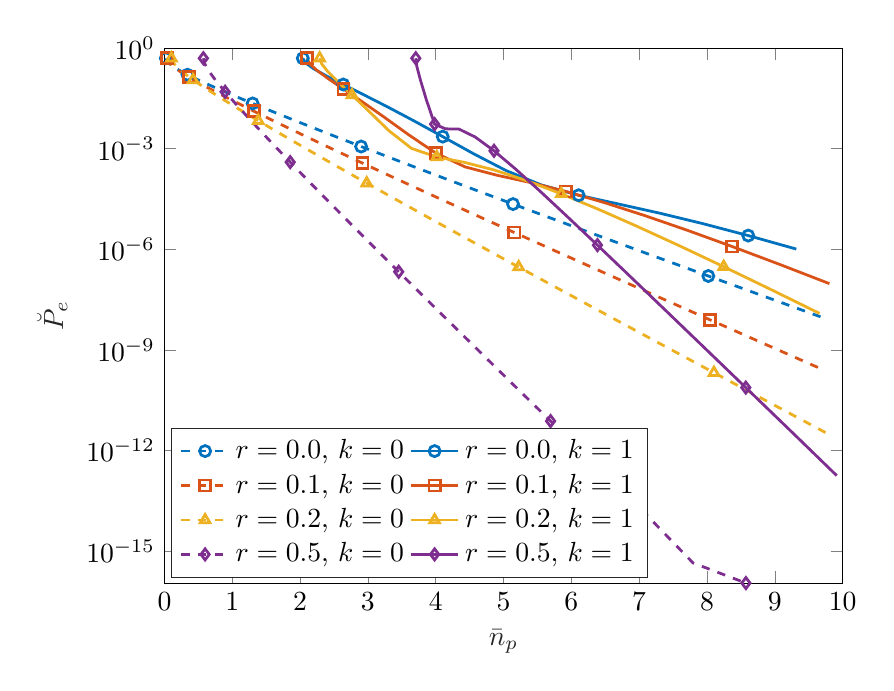
\begin{tikzpicture}

\begin{axis}[%
width=4.521in*0.75,
height=3.566in*0.75,
at={(0.758in,0.481in)},
scale only axis,
xmin=0,
xmax=10,
xlabel style={font=\color{white!15!black}},
xlabel={$\bar{n}_p$},
ymode=log,
ymin=1.11022302462516e-16,
ymax=1,
yminorticks=true,
ylabel style={font=\color{white!15!black}},
ylabel={$\breve{P}_e$},
axis background/.style={fill=white},
%axis x line*=bottom,
%axis y line*=left,
legend style={at={(0.01,0.01)}, anchor=south west, legend cell align=left, align=left, draw=white!15!black, legend columns=2}
]
\addplot [color=mycolor1, dashed, line width=1.0pt, mark=o, mark options={solid, mycolor1}, mark repeat={4}]
  table[row sep=crcr]{%
0.0200000000020406	0.5\\
0.0400000000020402	0.402886691283791\\
0.10000000000204	0.311248795396143\\
0.20000000000204	0.229705791588748\\
0.34000000000204	0.161367836859558\\
0.52000000000204	0.107527572164159\\
0.740000000002041	0.0677402706067528\\
1.00000000000204	0.040228893816313\\
1.30000000000204	0.0224701735043469\\
1.64000000000204	0.0117874985937501\\
2.02000000000204	0.00580411358757571\\
2.44000000000204	0.00268301603344689\\
2.90000000000204	0.00116504474732904\\
3.40000000000204	0.000475529564681332\\
3.94000000000204	0.00018252496091431\\
4.52000000000204	6.58942320924671e-05\\
5.14000000000204	2.2372962739603e-05\\
5.80000000000205	7.14262612222516e-06\\
6.50000000000204	2.14348977123358e-06\\
7.24000000000202	6.04459258424228e-07\\
8.02000000000186	1.60120172343348e-07\\
8.84000000000037	3.98308174776041e-08\\
9.69999999998796	9.30169952173543e-09\\
};
\addlegendentry{$r = 0.0$, $k = 0$}

\addplot [color=mycolor1, line width=1.0pt, mark=o, mark options={solid, mycolor1}, mark repeat={4}]
  table[row sep=crcr]{%
2.04000000000614	0.5\\
2.07980388157475	0.365238945696499\\
2.19695222552987	0.245075031520992\\
2.38527239346053	0.149666545304717\\
2.6362387582965	0.0824178394910576\\
2.94079284127565	0.0405450261122263\\
3.29080184759698	0.0176651515033895\\
3.67986533387235	0.0067767120762533\\
4.10351356897534	0.00229560228979309\\
4.55900917319244	0.000707434570884347\\
5.04497309453299	0.00021948919726017\\
5.56098876721283	8.28582489130203e-05\\
6.10726290808727	4.1022391904566e-05\\
6.68436781659824	2.27142595118912e-05\\
7.29306128054439	1.21004232845334e-05\\
7.93416896319587	5.8707409222869e-06\\
8.60851248045389	2.56977332785402e-06\\
9.31686877149291	1.01844033345566e-06\\
};
\addlegendentry{$r = 0.0$, $k = 1$}

\addplot [color=mycolor2, dashed, line width=1.0pt, mark=square, mark options={solid, mycolor2}, mark repeat={4}]
  table[row sep=crcr]{%
0.0404680907314567	0.5\\
0.0604680907314585	0.392901670542549\\
0.120468090731458	0.293128630573881\\
0.220468090731458	0.206620339442921\\
0.360468090731457	0.136941029534563\\
0.540468090731457	0.084941538631533\\
0.760468090731459	0.0491016108355734\\
1.02046809073146	0.026360899632598\\
1.32046809073146	0.0131130551179189\\
1.66046809073146	0.00603787611242568\\
2.04046809073146	0.00257369694341059\\
2.46046809073146	0.00101640450241469\\
2.92046809073146	0.000372205972558992\\
3.42046809073146	0.00012645461779881\\
3.96046809073146	3.98629468535416e-05\\
4.54046809073146	1.16575616797565e-05\\
5.16046809073146	3.16151968782208e-06\\
5.82046809073146	7.94771541634542e-07\\
6.52046809073146	1.85116668105501e-07\\
7.26046809073146	3.99314517562921e-08\\
8.04046809073146	7.97410959485489e-09\\
8.86046809073146	1.47367751335281e-09\\
9.72046809073146	2.51973775178271e-10\\
};
\addlegendentry{$r = 0.1$, $k = 0$}

\addplot [color=mycolor2, line width=1.0pt, mark=square, mark options={solid, mycolor2}, mark repeat={4}]
  table[row sep=crcr]{%
2.1016048937167	0.5\\
2.13722342176411	0.351557555027417\\
2.24231126096937	0.222160769918723\\
2.41204284470634	0.124222362453645\\
2.63974114418153	0.0603925042112791\\
2.91829336919182	0.0250484475022711\\
3.24129213294307	0.00872798119433771\\
3.60367379405264	0.00258598757293121\\
4.0018832937306	0.000741253402724129\\
4.43372687028477	0.000287093498001045\\
4.89808386454928	0.000162974574048513\\
5.39459822969919	9.8293093218349e-05\\
5.9234122263596	5.2962165794368e-05\\
6.48496287009384	2.48063685127087e-05\\
7.07983886502512	1.01844444848065e-05\\
7.70868661927138	3.70885692668743e-06\\
8.37215237665687	1.20946493997742e-06\\
9.07084922366429	3.55623495429391e-07\\
9.80534037124127	9.47534976036835e-08\\
};
\addlegendentry{$r = 0.1$, $k = 1$}

\addplot [color=mycolor3, dashed, line width=1.0pt, mark=triangle, mark options={solid, mycolor3}, mark repeat={4}]
  table[row sep=crcr]{%
0.102693819275224	0.5\\
0.122693819275224	0.381945077116474\\
0.182693819275225	0.273671210068553\\
0.282693819275225	0.18272455257\\
0.422693819275225	0.112952560216816\\
0.602693819275226	0.0642502792905548\\
0.822693819275224	0.03345396094764\\
1.08269381927522	0.0158838250522541\\
1.38269381927522	0.00686368066298626\\
1.72269381927522	0.00269897231763505\\
2.10269381927523	0.000966736234112642\\
2.52269381927523	0.000315777240763426\\
2.98269381927522	9.41232533182568e-05\\
3.48269381927522	2.56024275193667e-05\\
4.02269381927522	6.35315675889814e-06\\
4.60269381927523	1.43743867431212e-06\\
5.22269381927523	2.96354467355098e-07\\
5.88269381927523	5.5640574203597e-08\\
6.58269381927523	9.50809414534959e-09\\
7.32269381927523	1.47814516182621e-09\\
8.10269381927523	2.08976613791378e-10\\
8.92269381927523	2.68594035901515e-11\\
9.78269381927522	3.13798986795177e-12\\
};
\addlegendentry{$r = 0.2$, $k = 0$}

\addplot [color=mycolor3, line width=1.0pt, mark=triangle, mark options={solid, mycolor3}, mark repeat={4}]
  table[row sep=crcr]{%
2.28886800904409	0.5\\
2.31999800521609	0.335903697984307\\
2.41216418530892	0.196933331036258\\
2.56201679884254	0.0981076147304128\\
2.76489646890086	0.040185809256969\\
3.0158018679935	0.0130832203468926\\
3.31018324953374	0.00344887391962134\\
3.64440096753075	0.00101951363497232\\
4.01585991019939	0.000567040966715227\\
4.42292358106145	0.000392962039574174\\
4.86472316966757	0.000231481537813827\\
5.34094583218671	0.000111581978084918\\
5.85164780473884	4.51448958011524e-05\\
6.39710893432961	1.56946401249081e-05\\
6.97772869816361	4.76400489057838e-06\\
7.59395670680091	1.27574898745042e-06\\
8.24624906333657	3.03436716753147e-07\\
8.93504283030325	6.43988304904752e-08\\
9.66074253748888	1.2235391422255e-08\\
};
\addlegendentry{$r = 0.2$, $k = 1$}

\addplot [color=mycolor4, dashed, line width=1.0pt, mark=diamond, mark options={solid, mycolor4}, mark repeat={4}]
  table[row sep=crcr]{%
0.573942245572178	0.5\\
0.593942245028823	0.342499519674481\\
0.653942245170735	0.20790550335767\\
0.753942245341616	0.110057719920144\\
0.893942244583911	0.0500472584431716\\
1.07394224497389	0.0193143675146228\\
1.293942244546	0.00628332214973615\\
1.55394224371114	0.00172174882973891\\
1.85394224420503	0.000398395169961208\\
2.19394224278596	7.80046198984863e-05\\
2.57394224201761	1.29266966575337e-05\\
2.99394224220523	1.81130230003657e-06\\
3.45394223899107	2.14287482536157e-07\\
3.95394223844945	2.13728023612525e-08\\
4.49394223715584	1.79488168772224e-09\\
5.07394223021208	1.26788857190974e-10\\
5.693942230031	7.52714557350487e-12\\
6.35394222368679	3.74977826567147e-13\\
7.05394220748901	1.55431223447522e-14\\
7.79394220753813	4.44089209850063e-16\\
8.57394218450974	1.11022302462516e-16\\
9.39394214003978	0\\
};
\addlegendentry{$r = 0.5$, $k = 0$}

\addplot [color=mycolor4, line width=1.0pt, mark=diamond, mark options={solid, mycolor4}, mark repeat={4}]
  table[row sep=crcr]{%
3.7061308486222	0.5\\
3.72318775095693	0.276003723186423\\
3.77462452178882	0.111964236743116\\
3.86118165596315	0.0292098038693948\\
3.98392247081425	0.00541832505604978\\
4.14404207041508	0.00392337294658973\\
4.34269448841782	0.00386065139664005\\
4.58087300628471	0.00224591730584783\\
4.85935291484359	0.000870231139084243\\
5.17868537920139	0.000246879397142796\\
5.53922245734845	5.40728938508428e-05\\
5.94115678880561	9.42866109115981e-06\\
6.38456317979691	1.33219265713302e-06\\
6.86943477192184	1.54061789436888e-07\\
7.39571266351863	1.46675764867155e-08\\
7.96330772743687	1.15372272846415e-09\\
8.57211535637269	7.51390061282109e-11\\
9.22202638435226	4.05170341721828e-12\\
9.9129334474046	1.78523862359725e-13\\
};
\addlegendentry{$r = 0.5$, $k = 1$}
\end{axis}
\end{tikzpicture}%
                \caption{MDEP of noisy PASS quantum BPSK system as function of $\bar{n}_p$ with
                $N=40$, $\bar{n}=10^{-2}$, $\theta=\pi$ and $p_0=p_1=1/2$.}
                \label{fig:3.7}
            \end{center}
        \end{figure}